\begin{center}
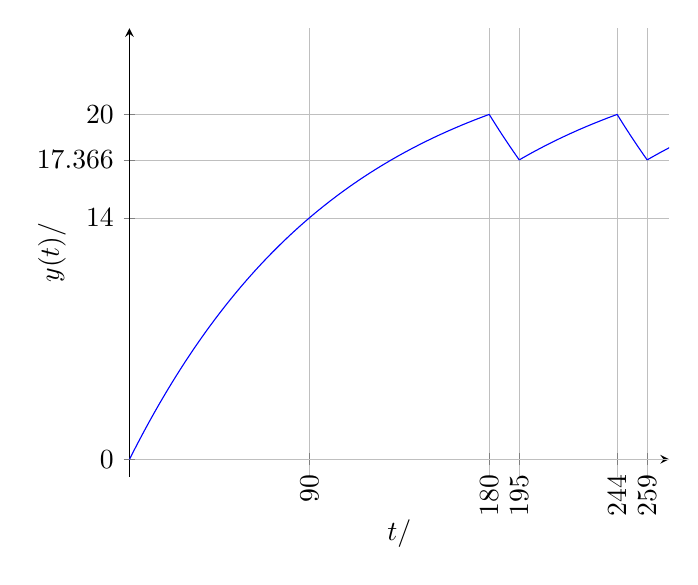
\begin{tikzpicture}
    \begin{axis}[
        domain=0:270,
        xmin=0, xmax=270,
        ymin=-1, ymax=25,
        samples=500,
        axis y line=center,
        axis x line=middle,
        %xtick distance=1,
        %ytick distance=1,
        extra y ticks=0,
        x label style={at={(axis description cs:0.5,-.075)},anchor=north},
        y label style={at={(axis description cs:-.1,.5)},rotate=90,anchor=south},
        xlabel={$t/\minute$},
        ylabel={$y(t)/\celsius$},
        ytick={0,14,17.366,20},
        xtick={0, 90, 180, 195,  244,  259},
        xticklabels={0, 90, 180, 195,  244,  259},
        xticklabel style={rotate=90},
        yticklabels={0,14,17.366,20},
        grid=both,
        grid style={line width=.1pt, draw=gray!10},
        major grid style={line width=.2pt,draw=gray!50},    ]
        \addplot+[color=blue,mark=none,domain=0:180] {2000*0.01225*(1-exp(-x/106.22))};
        \addplot+[color=blue,mark=none,domain=180:195] {20*(exp(-(x-180)/106.22))};
        \addplot+[color=blue,mark=none,domain=195:244] {2000*0.01225*(1-exp(-(x-64)/106.22))};
        \addplot+[color=blue,mark=none,domain=244:259] {20*(exp(-(x-244)/106.22))};
        \addplot+[color=blue,mark=none,domain=259:300] {2000*0.01225*(1-exp(-(x-128)/106.22))};
    \end{axis}
\end{tikzpicture}
\end{center}